\documentclass[12pt,dvipsnames,aspectratio=169]{beamer}

\usepackage[french]{babel}
\usepackage[T1]{fontenc}
\usepackage[utf8]{inputenc}
\usepackage{xcolor}
\usepackage{ragged2e}
\usepackage{amsmath, amsthm, amssymb, latexsym}
\usepackage{derivative}
\usepackage{graphicx, animate} % Required for inserting images
\usepackage{transparent} % Image transparency
\usepackage{tikz}

\graphicspath{{./figures}}

% ----- Beamer theme -----
\usetheme{Singapore}
\usecolortheme{lily}
\usefonttheme{professionalfonts}
\useinnertheme{circles}

% ----- Beamer template -----

% Remove color boxes around title and header
\setbeamercolor{section in head/foot}{bg=white}
\setbeamercolor{subsection in head/foot}{bg=white}
\setbeamercolor{subsubsection in head/foot}{bg=white}
\setbeamercolor{titlelike}{bg=white, fg=black}

% Left align frame titles
\setbeamertemplate{frametitle}
{
    \usebeamerfont{frametitle}\insertframetitle\par
    \usebeamerfont{framesubtitle}\insertframesubtitle\par
}

% Footer
\setbeamertemplate{navigation symbols}{} % Remove navigation symbols
\makeatother
\setbeamertemplate{footline}
{
  \leavevmode%
  \hbox{%
  \begin{beamercolorbox}[wd=\paperwidth,ht=2.25ex,dp=1ex,sep=1ex,center]{title in head/foot}%
    \usebeamerfont{title in head/foot}ENSC 2A --- Apprentissage Automatique CM5
    \hfill
    \insertframenumber{} / \inserttotalframenumber
  \end{beamercolorbox}
  }%
  \vskip0pt%
}
\makeatletter

% Title frame
\setbeamertemplate{title page}
{
    \vspace{1em}
    \begin{beamercolorbox}[wd=10cm]{}
        \usebeamerfont{institute}ENSC 2A --- Apprentissage Automatique CM5%
    \end{beamercolorbox}
    \vspace{1.5em}
    \begin{beamercolorbox}[wd=\paperwidth,center]{}
        \begin{figure}
            \centering
            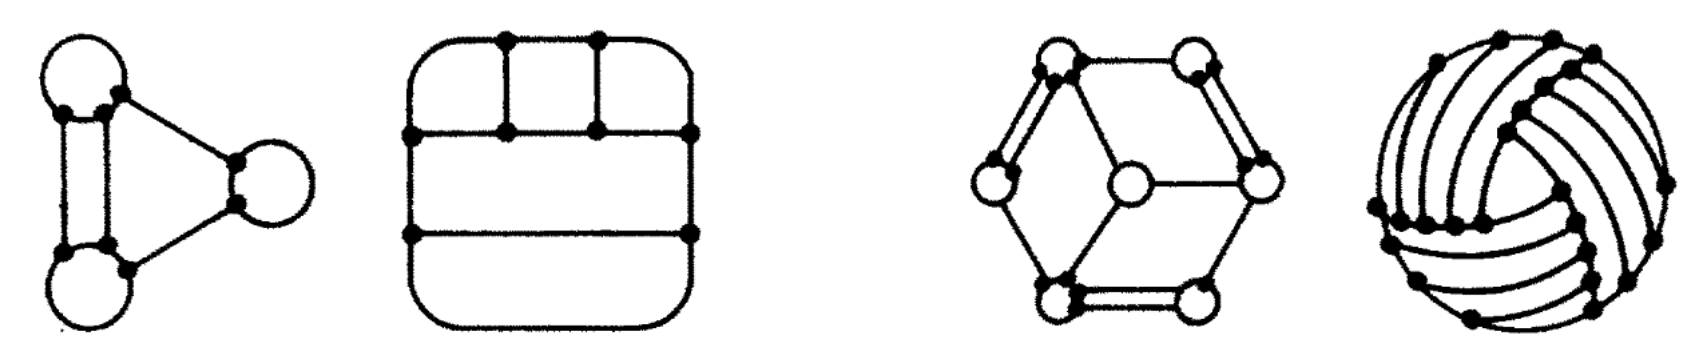
\includegraphics[width=\textwidth]{minsky63.png}
        \end{figure}
    \end{beamercolorbox}
    \vspace{1.5em}
    \begin{beamercolorbox}[wd=10cm]{title page header}
        \usebeamerfont{title}\inserttitle\par%
    \end{beamercolorbox}
    \vspace{0.5em}
    \begin{beamercolorbox}[wd=5cm]{author}
        \usebeamerfont{author}\insertauthor\par%
    \end{beamercolorbox}
    \vspace{0.3em}
    \begin{beamercolorbox}[wd=5cm]{}
        \usebeamerfont{institute}\insertinstitute\par%
    \end{beamercolorbox}
    \begin{beamercolorbox}[wd=\paperwidth,right,sep=1em]{}
        \tiny{\emph{Image adaptée de Minsky (1961), Proc. IRE}}
    \end{beamercolorbox}
}

% ----- Metadata -----
\title{Entraînement de Réseaux de Neurones Artificiels}
\author{Nathan Trouvain}
\institute[Inria] % (optional)
{
  Inria Mnemosyne\\%
  nathan.trouvain@inria.fr\\%
}
\date{February 2024}

% ----- Utils -----

\newcommand{\xset}[0]{\mathcal{X}}
\newcommand{\x}[0]{\mathbf{x}}
\newcommand{\X}[0]{\mathbf{X}}
\newcommand{\yset}[0]{\mathcal{y}}
\newcommand{\y}[0]{\mathbf{y}}
\newcommand{\Y}[0]{\mathbf{Y}}
\newcommand{\w}[0]{\mathbf{w}}
\newcommand{\f}[1]{f^{(#1)}_{\theta_{#1}}}
\newcommand{\hl}[0]{\mathbf{h}_l}
\newcommand{\hli}[0]{\mathbf{h}_{l-1}}
\newcommand{\al}[0]{\mathbf{a}_{l}}
\newcommand{\ali}[0]{\mathbf{a}_{l-1}}

% ----- Slides ------

\AtBeginSection[]{
  \frame<beamer>{ 
    \frametitle{Sommaire}   

\tableofcontents[currentsection,sectionstyle=show/shaded]}
}

\begin{document}

\begin{frame}[plain]
    \maketitle
\end{frame}

\begin{frame}{Sommaire}
    \setcounter{tocdepth}{1}
    \tableofcontents
\end{frame}

\section{Optimisation de modèles paramétriques (rappels)}

% \begin{frame}{Modèles statistiques}{Rappels}

%     \begin{columns}
%         \column{0.6\textwidth}
%             \begin{block}{Définition}
%                 \justifying
%                 Un modèle statistique est un modèle mathématique qui \textbf{met en application un certain nombre d'hypothèses statistiques concernant la génération d'un jeu de données}; il permet d'expliquer, de manière idéalisée, le processus de génération de ces données.
%             \end{block}
%         \column{0.4\textwidth}
%             \begin{exampleblock}{Exemple}
%                 Soient $X \sim p(X)$,\par
%                 $Y \sim q(Y)$,\par
%                 $(w, b) \in \mathbb{R}^2$:\par
%                 \begin{equation*}
%                     Y = w \cdot X + b
%                 \end{equation*}

%                 est un modèle expliquant la relation affine entre $X$ et $Y$.
%             \end{exampleblock}
%     \end{columns}
    
% \end{frame}

% \begin{frame}{Modèles statistiques}{Notations}
%     \begin{columns}
%         \column{0.6\textwidth}
%             Plusieurs hypothèses possibles ici:
%             \begin{itemize}
%                 \item<1->Relation linéaire entre $X$ et $Y$
%                 \item<2->Forme de $p(X)$
%                 \item<3->Forme de $p(Y)$
%                 \item<4->Distribution de $w$ et $b$
%             \end{itemize}
%         \column{0.4\textwidth}
%             \begin{exampleblock}{Exemple}
%                 Soient $X \sim p(X)$,\par
%                 $Y \sim q(Y)$,\par
%                 $(w, b) \in \mathbb{R}^2$:\par
%                 \begin{equation*}
%                     Y = w \cdot X + b
%                 \end{equation*}
%             \end{exampleblock}
%     \end{columns}
% \end{frame}

% \begin{frame}{Apprentissage supervisé}{Principe}
%     Données: $(X, Y) = \{(\x_1, \y_1), (\x_2, \y_2), \dots (\x_n, \y_n)\}$\par
%     Paramètres inconnus $\mathbf{\Theta} = \{\theta_1, \theta_2, \dots \theta_m\}$\par
%     \pause
%     \begin{block}{Objectif}
%         Trouver $\y = f(\x; \Theta)$
%         \pause
%         \begin{figure}
%             \centering
%             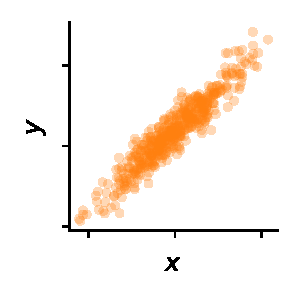
\includegraphics[width=0.4\textwidth]{linear.pdf}
%             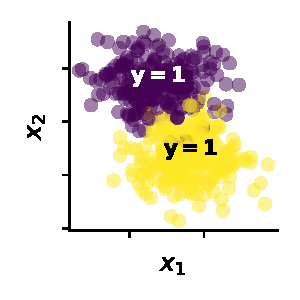
\includegraphics[width=0.4\textwidth]{blobs.pdf}
%         \end{figure}
%     \end{block}
% \end{frame}

% \begin{frame}{Apprentissage supervisé}{Objectif}
%     \begin{block}{Objectif}
%         Trouver $\y = f(\x; \Theta)$ \pause $\rightarrow$ Maximiser $\underbrace{P(Y | X, \Theta)}_{\text{\alert{Vraisemblance \textit{(Likelihood)}}}}$
%     \begin{itemize}
%         \item $(X, Y)$ sont toutes observations
%         \item $f$, $\Theta$ sont nos hypothèses
%     \end{itemize}
%     \textbf{$\rightarrow$ Trouver les hypothèses les plus probables expliquant $Y$ à partir de $X$.}
%     \end{block}
% \end{frame}

% \begin{frame}{Apprentissage supervisé}{Objectif}
%     \begin{exampleblock}{Exemple}
%         \begin{columns}
%             \column{0.5\textwidth}
%             \begin{figure}
%                 \centering
%                 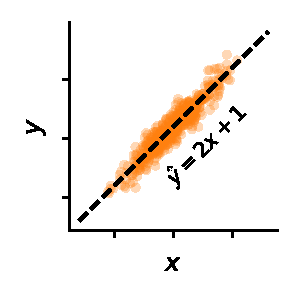
\includegraphics[width=\textwidth]{figures/linear_explained.pdf}
%             \end{figure}
%             \column{0.5\textwidth}
%             Hypothèse la plus probable pour expliquer $Y$: 
%             $$y = w \cdot x + b$$\par
%             avec $\Theta = (w, b) = (2, 1)$

%             Peut aussi se formuler:
%             $$Y \sim \mathcal{N}(wX+b, \sigma^2)$$
%             où $\sigma^2$ demeure un paramètre indéterminé.
%         \end{columns}
%     \end{exampleblock}
    
% \end{frame}

\begin{frame}{Modèles statistiques}{Rappels}

    \begin{block}{Définition}
        \justifying
        Un modèle statistique est un modèle mathématique qui \textbf{met en application un certain nombre d'hypothèses statistiques concernant la génération d'un jeu de données}; il permet d'expliquer, de manière idéalisée, le processus de génération de ces données.
    \end{block}
    
\end{frame}


\begin{frame}{Modèles statistiques}{Notations}

    \begin{table}[]
        \centering
        \begin{tabular}{ll}
             $X$ & variables aléatoires observées \\
             $\x_i = [x_{i,1}, x_{i,2}, \dots x_{i,p}]$ & observation $i$ ($p$ variables) \\
             $\X = [\x_1, \x_2, \dots \x_n]$ & matrice de $n$ observations ($n \times p$)\\
             & \\
             Idem pour $Y$, $\y_i$, $\Y$ & variables/observations cibles \\
             & \\
             $\Theta = \{\theta_1, \theta_2, \dots \theta_m\}$ & tous les paramètres d'un modèle
        \end{tabular}
    \end{table}

    \textbf{But: trouver $f, \Theta$ tels que $f_\Theta(\x) = \y$.}

    \textbf{$f_\Theta$ est notre modèle.} Il implémente nos hypothèses ($f, \Theta$).

\end{frame}

\begin{frame}{Modèles statistiques}{Exemple}
    \begin{columns}
        \column{0.5\textwidth}
        \begin{figure}
            \centering
            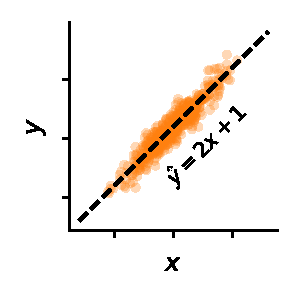
\includegraphics[width=\textwidth]{figures/linear_explained.pdf}
        \end{figure}
        \column{0.5\textwidth}
        Hypothèse la plus probable pour expliquer $Y$ à partir de $X$: 
        $$Y = w \cdot X + b$$\par
        avec $\Theta = (w, b) = (2, 1)$ et $f$ une fonction affine.
    \end{columns}
\end{frame}

\begin{frame}{Apprentissage supervisé}{Objectif général}
    \begin{block}{Apprentissage supervisé}
        Processus permettant de déterminer automatiquement $\Theta$ à partir d'observations $(\X, \Y)$, en supposant $f$.
    \end{block}

    \begin{block}{Nécessaire}
        \begin{itemize}
            \item \textbf{un modèle} $\rightarrow$ \textit{quel type d'hypothèses je vais faire ?}
            \item \textbf{une fonction d'objectif} $\rightarrow$ \textit{à quel point mon hypothèse est valide ?}
            \item \textbf{un algorithme permettant de minimiser/maximiser cette objectif} $\rightarrow$ \textit{comment poser une meilleure hypothèse ?}
        \end{itemize}
    \end{block}
\end{frame}

\begin{frame}{Apprentissage supervisé}{Dans le cadre de ce cours}
    \begin{block}{Apprentissage supervisé}
        Processus permettant de déterminer automatiquement $\Theta$ les plus probables à partir d'observations $(\X, \Y)$, en supposant $f$.
    \end{block}
    
    \begin{block}{Nécessaire}
        \begin{itemize}
            \item \textbf{un modèle} $\rightarrow$ \textit{\alert{Perceptron multicouche}} (approximateurs universels)
            \item \textbf{une fonction d'objectif} $\rightarrow$ \textit{\alert{Loss}}
            \item \textbf{un algorithme permettant de minimiser/maximiser cette objectif} $\rightarrow$ \textit{\alert{Descente de gradient}}
        \end{itemize}
    \end{block}
\end{frame}

\begin{frame}{Rappels: perceptron multicouche}{Notations et définition}

    Perceptron simple avec $\theta = \{\w, b\}$ et fonction d'activation $\sigma$:
    \begin{equation*}
        f_\theta(\x) = \sigma(\sum_i^p w_i x_i + b) = \sigma(\w^\intercal \cdot \x + b)
    \end{equation*}

    \begin{figure}
        \centering
        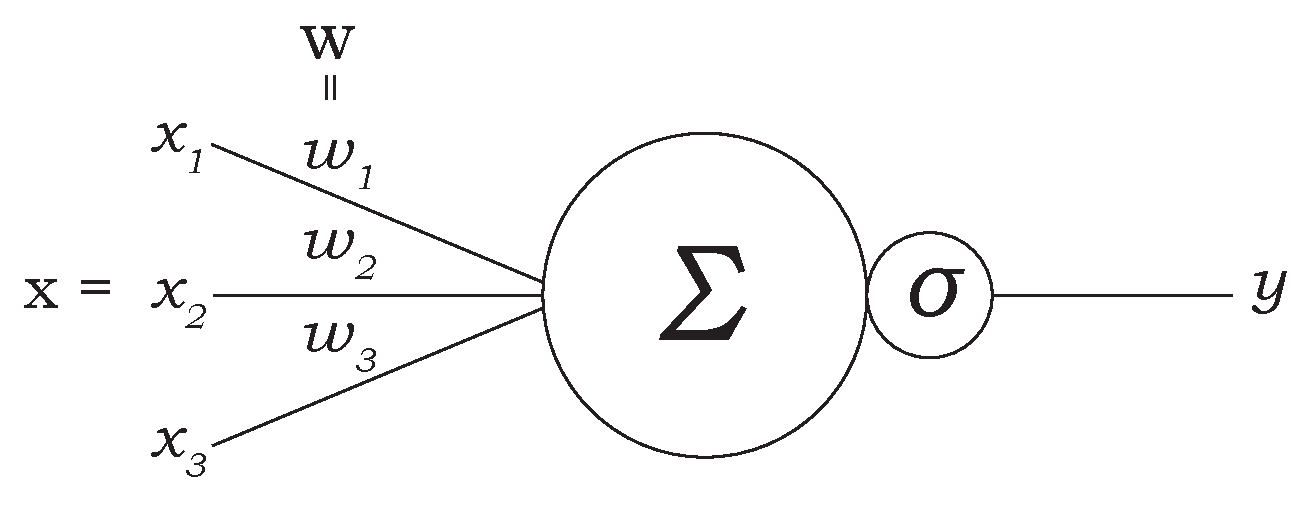
\includegraphics[width=0.6\textwidth]{figures/perpcetron.pdf}
    \end{figure}

\end{frame}

\begin{frame}{Rappels: perceptron multicouche}{Notations et définition}

    \begin{columns}

        \column{0.5\textwidth}
            Perceptron multicouche avec $L$ couches de perceptrons $(\f{i})_{i=0 \dots L}$ et $\Theta = \{\theta_1, \dots \theta_L\}$ :
    \begin{align*}
        F_\Theta(\x) &= f_{\theta_l}^{(l)}(f_{\theta_{l-1}}^{(l-1)}(\dots f^{(1)}_{\theta_1}(\x))) \\
                 &= \f{l} \circ \f{l-1} \circ \dots \circ \f{1}(\x)
    \end{align*}

    \column{0.5\textwidth}
    \begin{figure}
        \centering
        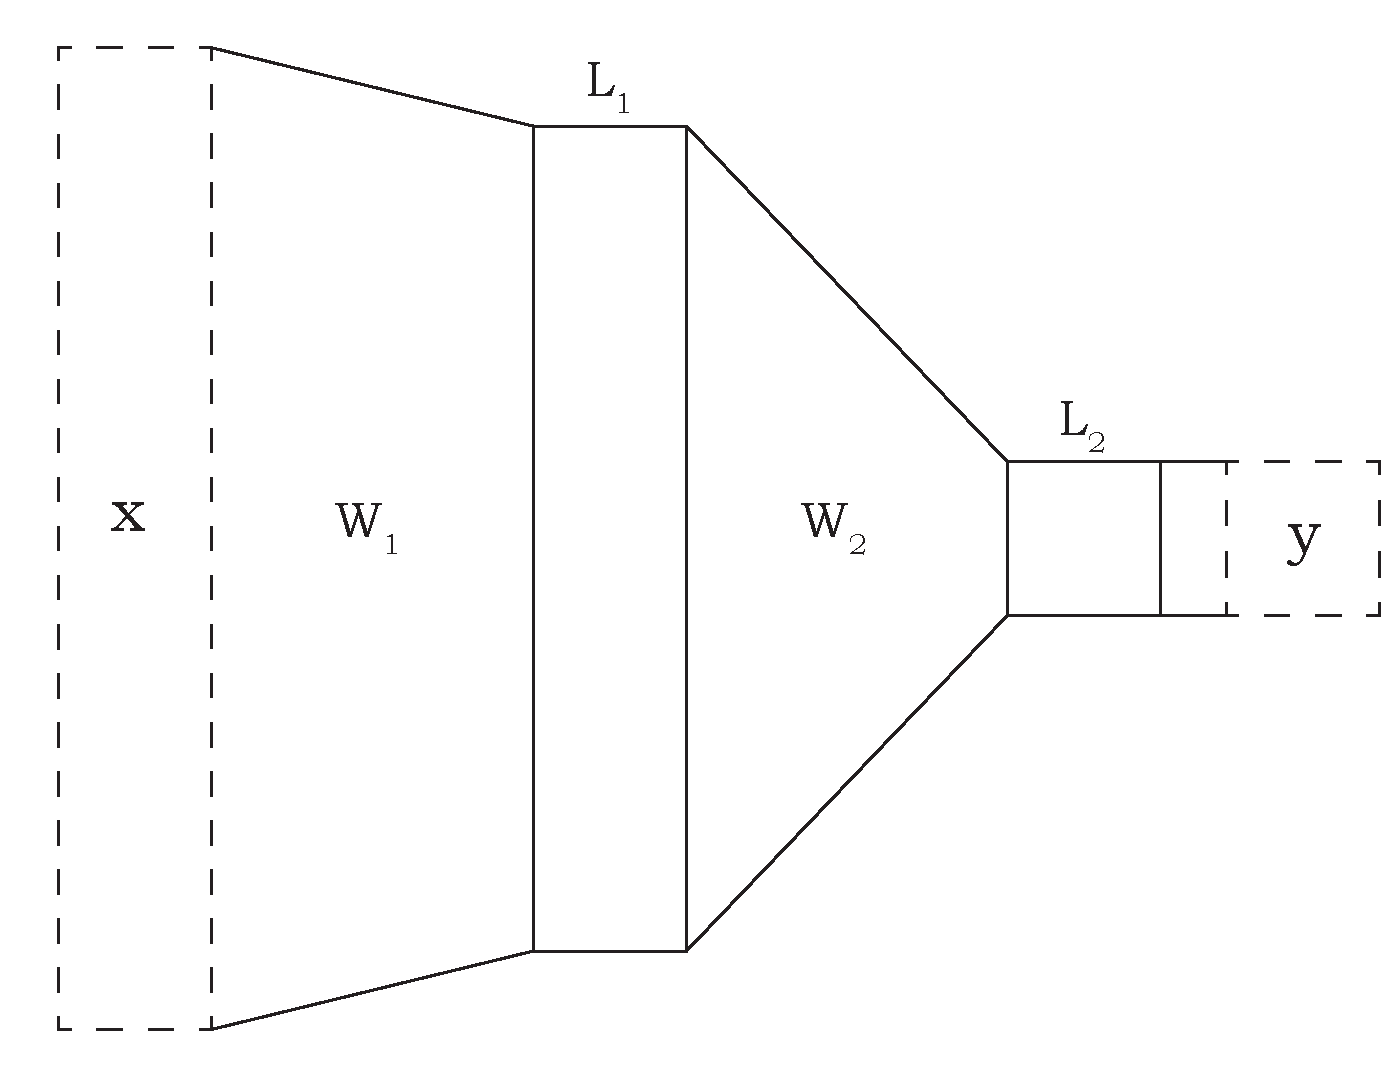
\includegraphics[width=\textwidth]{figures/mlp.pdf}
    \end{figure}
    \end{columns}


\end{frame}

\begin{frame}{Rappels: \textit{Loss}}{C'est quoi, en fait ?}

    \begin{block}{But de l'optimisation}
        Minimiser \textbf{une fonction d'objectif (ou \textit{loss})} $\ell(\Theta)$;\par
        $\ell(\Theta)$ est \textbf{convexe} (a un minimum) et  est \textbf{continue et différentiable} (on peut glisser jusqu'à ce minimum sans problème). \textbf{Le minimum de $\ell({\Theta})$ nous indique quels $\Theta$ répondent le mieux à la tâche fixée sur les données disponibles.}
    \end{block}

\end{frame}

\begin{frame}{Rappels: \textit{Loss}}{C'est quoi, en fait ?}
\begin{figure}
    \centering
    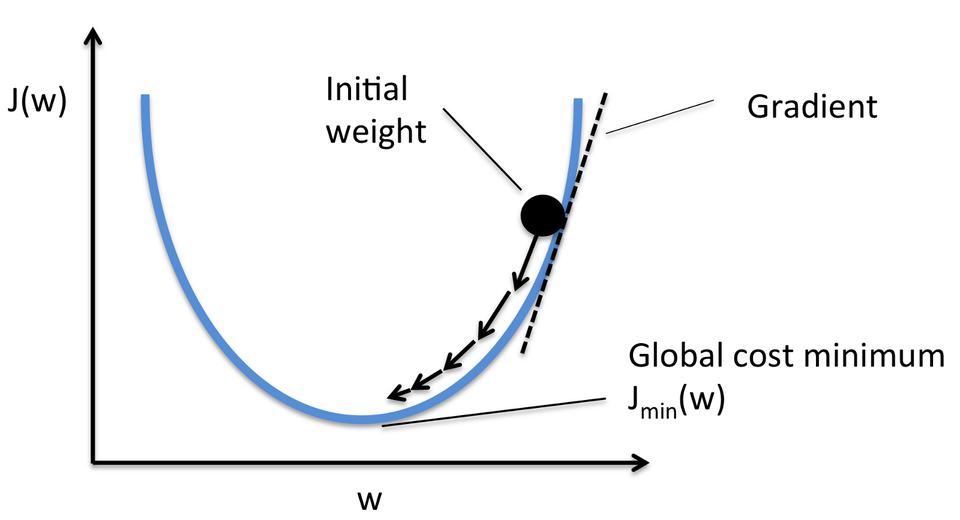
\includegraphics[width=0.8\textwidth]{gradient_descent_1parameter.png}
\end{figure}
\end{frame}

\begin{frame}{Rappels: \textit{Loss}}{C'est quoi, en fait ?}

    \begin{block}{Remarque (hors cadre du cours)}
        Souvent, en pratique, $\ell(\Theta) = E(\Theta) + R(\Theta)$

        \vspace{1em}
        
        $E$ est une \textbf{fonction d'erreur} (à quel distance je suis des prédictions souhaitées ?) et $R$ est une \textbf{fonction de régularisation} (quel est le modèle le plus simple pour y parvenir ?).\par
        Par exemple, $R(\Theta) = ||\Theta||^2$ (régularisation $\ell_2$ ou \textit{ridge}).

    \end{block}

\end{frame}

\begin{frame}{Rappels: \textit{Loss}}{C'est quoi, en fait ?}
    \begin{table}[]
        \centering
        \begin{tabular}{c|c}
             \textbf{Tâche} & \textbf{\textit{Loss} canonique} \\
             Régression & \textit{Mean Squared Error} \\
             Classification (2 classes) & \textit{Binary crossentropy} \\
             Classification ($k$ classes) & \textit{Crossentropy} \\
             \dots & \dots
        \end{tabular}
    \end{table}

    \begin{block}{Remarque}
        En pratique, la fonction d'objectif (ou \textbf{\textit{loss}}, ou encore \textit{cost}) utilisée pour l'apprentissage dans les réseaux de neurones est souvent issue de la \textit{negative log-likelihood} (moins le log de la vraissemblance).
    \end{block}

    
\end{frame}

\begin{frame}{(Plus vraiment des) Rappels: \textit{Likelihood}}{C'est quoi, en fait ?}

    \begin{exampleblock}{Exemple: objectif pour la classification}
        Soit $X$ un ensemble d'images de chats ou de chiens, et $Y$ un ensemble de labels valant $1$ pour les chats et $0$ pour les chiens. On souhaite estimer $p = P(Y=1|X)$, la probabilité qu'une image soit un chat. On définit un modèle tel que $p = f_\Theta(\x)$.
        
        \textbf{Objectif: avoir la meilleure estimation de $p$ par $f_\Theta$ sachant n'importe quel $\x$.}
    \end{exampleblock}

\end{frame}


\begin{frame}{(Plus vraiment des) Rappels: \textit{Likelihood}}{C'est quoi, en fait ?}

    \begin{exampleblock}{Exemple: objectif pour la classification}
        \textbf{Objectif: avoir la meilleure estimation de $p$ par $f_\Theta$ sachant n'importe quel $\x$.}

        \begin{align*}
            P(Y=1 \text{~(chat)}|X=\x) &= p = f_\Theta(\x) \\
            P(Y=0 \text{~(chien)}|X=\x) &= 1-p = 1-f_\Theta(\x) \\
            \implies P(Y=k|X) &= p^k(1-p)^k \text{~~(loi de Bernoulli)} 
        \end{align*}
    \end{exampleblock}

\end{frame}


\begin{frame}{(Plus vraiment des) Rappels: \textit{Likelihood}}{C'est quoi, en fait ?}

        On définit la \textbf{likelihood (vraissemblance)} comme \textbf{la probabilité que les données observées soient issues du modèle $f_\Theta$}:
        \begin{align*}
            \mathcal{L}(\Theta) &= P(Y_1=\y_1, \dots Y_n=\y_n|X=\x_1, \dots X=\x_n) \\
            &\overset{iid}{=} \prod_i^n \underbrace{P(Y_i=\y_i|X=\x_i)}_{\text{dépend de } \Theta} \\
            &= \prod_i^n f_\Theta(\x_i)^{\y_i}(1 - f_\Theta(\x_i))^{\y_i}
        \end{align*}
        
\end{frame}


\begin{frame}{(Plus vraiment des) Rappels: \textit{Likelihood}}{C'est quoi, en fait ?}

    \begin{exampleblock}{Exemple: objectif pour la classification}
        On cherche donc \textbf{des valeurs de $\Theta$ qui maximisent la vraissemblance}:

        $$\underset{\Theta}{\mathrm{argmax}} ~ \mathcal{L}(\Theta)$$

        Pour simplifier les calculs (et éviter de multiplier des probabilités très faibles ensembles), on définit \textbf{une \textit{loss} équivalente à minimiser, la \textit{negative log-likelihood}} $\ell(\Theta)$:

        $$\underset{\Theta}{\mathrm{argmin}} ~ \ell(\Theta) = \mathbb{E}[-\ln \mathcal{L}(\Theta)]$$

    \end{exampleblock}

\end{frame}

\begin{frame}{(Plus vraiment des) Rappels: \textit{Likelihood}}{C'est quoi, en fait ?}

    \begin{exampleblock}{Exemple: objectif pour la classification}

        \begin{align*}
            \ell(\Theta) &= \mathbb{E}[-\ln \mathcal{L}(\Theta)] \\
            &= - \frac{1}{n} \sum_i^n \ln P(Y_i=\y_i|X=\x_i) \\
            &= - \frac{1}{n} \sum_i^n \y_i\ln(f_\Theta(\x_i)) + (1-\y_i)\ln(f_\Theta(\x_i))
        \end{align*}

        On appelle cette \textit{loss} une \textbf{entropie croisée binaire} (\textit{binary crossentropy}).

    \end{exampleblock}

\end{frame}

\begin{frame}{(Plus vraiment des) Rappels: \textit{Likelihood}}{C'est quoi, en fait ?}

    \begin{exampleblock}{Autres objectifs --- Exercices}

        De la même manière, on peut démontrer que:
        \begin{itemize}
            \item la \textit{loss} issue d'un objectif de maximisation de la vraissemblance sur une tâche de régression (avec cette fois-ci $P(Y|X) \sim \mathcal{N}(f_\Theta(X), \sigma^2)$) est \textbf{l'erreur quadratique moyenne} (\textit{mean squared error} a.k.a. MSE).
            \item la \textit{loss} issue du même objectif sur une tâche de classfication multiclasse (plus de 2 classes) donne \textbf{l'entropie croisée} (\textit{crossentropy}).
        \end{itemize}


    \end{exampleblock}

\end{frame}

\begin{frame}{Rappels: descente de gradient}{It's all coming together}

Trouver le meilleur modèle $f_\Theta$ qui prédit la valeur de $Y$ sachant $X$ \par
$\Rightarrow$ Trouver le minimum de la \textit{loss} $\ell(\Theta)$ \par
$\Rightarrow$ Trouver un point $\Theta^*$ tel que $\frac{d\ell}{d\Theta}(\Theta^*) = 0$

\vspace{1em}

\textbf{Solution}: descendre la pente de $\ell$, donc sa dérivée $\frac{d\ell}{d\Theta}$, jusqu'à s'approcher suffisamment d'un $\Theta^*$ intéressant.

<<video descente de gradient>>

\end{frame}


\begin{frame}{Problématique: \textit{credit assignment problem}}{Marvin Minsky, Seymour Papert, 1969: prémices de l'hiver de l'IA}

\small{(Nous sommes en 1969, la descente de gradient est encore un art mathématique obscur.)}

Dans un modèle profond, \textbf{calculer la contribution de chaque paramètre $\theta_i$ à la réponse finale du modèle est non trivial}.

\begin{exampleblock}{Exemple}
    Par exemple, dans le modèle:
    $$y = wx + b$$
    il est évident que $w$ définit la contribution de la variable $x$ au résultat final. La \textit{loss} peut-être minimisée analytiquement.
    Mais dans un modèle profond, cette contribution n'est plus évidente :
    $$y = f_2(w_2f_1(w_1x + b_1)+b_2)$$
\end{exampleblock}


\end{frame}

\begin{frame}{Problématique: \textit{credit assignment problem}}{Marvin Minsky, Seymour Papert, 1969: prémices de l'hiver de l'IA}
\textit{“In playing a complex game such as chess or checkers, or in writing a computer program, one has a definite success criterion – the game is won or lost. But in the course of play, each ultimate success (or failure) is associated with a vast number of internal decisions. If the run is successful, how can we assign credit for the success among the multitude of decisions?"}

--- Minsky, 1963

\end{frame}


\begin{frame}{Solution: la \textit{rétropropagation du gradient d'erreur}}{Seppo I. Linnainmaa, 1970; Paul Werbos, 1974; David E. Rumelhart, Geoffrey E. Hinton \& Ronald J. Williams, 1986}

Calculer, pour tous les $\Theta = \{\theta_1, \dots \theta_m\}$, le \textbf{gradient} (vecteur de dérivées partielles) de $\ell(\Theta)$ $\Rightarrow$ \textbf{calculer implicitement la contribution de chaque paramètre}:

$$
\nabla_\Theta\ell = \begin{bmatrix}
                        \pdv{\ell}{\theta_1} \\
                        \pdv{\ell}{\theta_2} \\
                        \vdots \\
                        \pdv{\ell}{\theta_m}
                    \end{bmatrix}
$$

Appliquer chaque dérivée partielle au $\theta_i$ correspondant (descente de gradient):

$$
\theta_i := \theta_i - \eta \nabla_\Theta\ell
$$

\end{frame}


\section{Algorithme de rétropropagation}

\begin{frame}{Préliminaires}{Notations}

Soit un perceptron multicouche $F_\Theta$, composé de $L$ couches, avec $\Theta = \{\w_1, \w_2 \dots \w_L, b_1, b_2, \dots b_L\}$, l'ensemble des paramètres. Soit $\hl$ la sortie d'une couche $l$ \textbf{avant activation} et $\al$ \textbf{après activation}:

\begin{align*}
    \hl &= \w \cdot \hli + b \\
    \al &= \sigma(\hl)
\end{align*}

\textbf{Remarque}: Si $l=1$ (entrée du réseau), alors $\hli=\x$.
    
\end{frame}

\begin{frame}{Préliminaires}{Notations}

Soit une fonction objectif $\ell({\Theta})$ quelconque, qu'on suppose continue et différentiable. On souhaite ici qu'elle calcule l'erreur commise entre une valeur souhaitée $\y$ et une valeur prédite par la dernière couche du réseau $\hat{\y} = \mathbf{a}_L$:

\begin{equation*}
    \ell({\Theta}) = err(\hat{\y}, \y) = err(\mathbf{a}_L, \y)
\end{equation*}

\end{frame}


\begin{frame}{Règle de chaînage}{LA DIAPO LA PLUS IMPORTANTE DU COURS}

En considérant toutes les fonctions impliquées comme \textbf{différentiables}, on peut écrire les dérivées partielles de l'erreur par rapport à chaque paramètre $i$ de chaque couche $l$ ($\theta_{l, i}$) que l'on note $\pdv{\ell}{\theta_{l, i}}$.

Cette valeur est directement calculable par la \textbf{règle de chaînage des dérivées}:

\begin{equation*}
    (f \circ g)'(x) = f'(g(x)) \cdot g'(x) = \odv{f}{g} \cdot \odv{g}{x}
\end{equation*}

\begin{equation*}
    \pdv{\ell}{\theta_{l, i}} = \pdv{\ell}{\mathbf{a}_L} \cdot \pdv{\mathbf{a}_L}{\mathbf{h}_L} \dots \pdv{\mathbf{a}_{l+1}}{\mathbf{h}_{l+1}} \cdot \pdv{\mathbf{h}_{l+1}}{\al} \cdot \pdv{\al}{\hl} \cdot \pdv{\hl}{\theta_{l, i}}
\end{equation*}

$\rightarrow$ Comme passer une donnée dans le réseau, mais \textbf{à l'envers}.

\end{frame}

\begin{frame}{Application}{Apprentissage en trois étapes}

    \begin{block}{1. \textit{Forward pass}}
    
        Calculer tous les $\hl$ et $\al$ couche par couche, à partir d'une donnée $\x$ soit \textbf{émettre une prédiction avec le réseau}.\par
        Calculer $\ell({\Theta})$, l'erreur commise avec les paramètres actuels.
        
    \end{block}
    
\end{frame}

\begin{frame}{Application}{Apprentissage en trois étapes}

    \begin{block}{2. \textit{Backward pass}}
    
        En partant de la valeur $\ell({\Theta})$ calculée, passer dans le réseau \textbf{à l'envers} pour calculer la contribution de chaque paramètre à cette valeur, soit \textbf{calculer la dérivée de l'erreur par rapport à chaque paramètres}.\par
        On applique pour ce faire la règle de chaînage. \par
        
    \end{block}
    
\end{frame}


\begin{frame}{Application}{Apprentissage en trois étapes}

    \begin{block}{3. Descente de gradient}
    
        Pour terminer, on applique l'algorithme de descente de gradient pour mettre à jour les paramètres avec les gradients calculés pendant la \textit{backward pass}.
        
    \end{block}
    
    \begin{block}{Puis retour à 1.}
    
        Recommencer avec un nouveau point ou groupe de points de donnée $\x$ \textbf{jusqu'à convergence} $\rightarrow$ jusqu'à ce que $\ell(\Theta)$ ne se réduise plus à chaque mise à jour des $\Theta$.
    \end{block}
    
\end{frame}

\begin{frame}{Application}{Apprentissage en trois étapes}

\begin{figure}
    \centering
    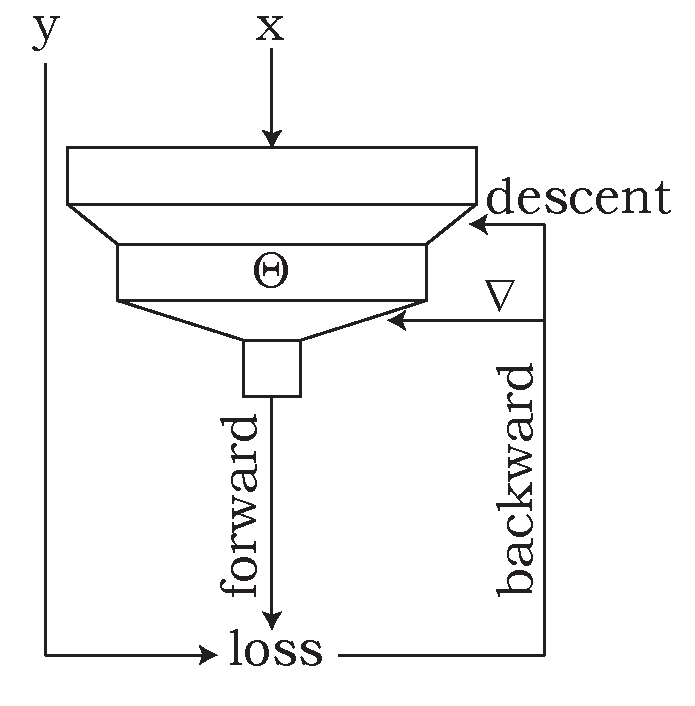
\includegraphics[width=0.4\textwidth]{figures/forwardbackward.pdf}
\end{figure}
    
\end{frame}


\begin{frame}{Exemple}{Forward pass}

    On se propose d'effectuer une tâche de régression sur un jeu de données $(\X, \Y) = (x_i, y_i)_{i=1\dots n}$ de taille $n$, avec $\dim x_i = 1 = \dim y_i$.

    Soit un perceptron multicouche $\hat{y} = F(x)$ à 3 couches, chacune contenant un unique neurone, équipées d'une fonction d'activation sigmoïde $\sigma(x) = \frac{1}{1 + e^{-x}}$, $\odv{\sigma}{x} = \sigma(x)(1-\sigma(x))$ ou identité $Id(x) = x$ pour la dernière couche.

    \begin{columns}
     \column{0.33\textwidth}
     \begin{center}
        Couche $l=1$
         \begin{align*}
            h_1 &= w_1 x + b_1 \\
            a_1 &= \sigma(h_1)
        \end{align*}
     \end{center}
     \column{0.33\textwidth}
     \begin{center}
      Couche $l=2$
     \begin{align*}
        h_2 &= w_2 a_1 + b_2 \\
        a_2 &= \sigma(h_2)
     \end{align*}
     \end{center}
     \column{0.33\textwidth}
     \begin{center}
      Couche $l=3$
     \begin{align*}
        h_3 &= w_3 a_2 + b_3 \\
        \hat{y} &= a_3 = Id(h_3)
     \end{align*}
     \end{center}
 \end{columns}

\end{frame}


\begin{frame}{Exemple}{Forward pass}

    Pour un point (ou un groupe de points) de données $x$, on calcule les $h_l$ et $a_l$.\par
    A la fin de la \textit{forward pass}, on calcule une dernière fonction, la \textit{loss}, dépendante de la sortie du réseau et donc de ses paramètres $\Theta$.
    
    \begin{equation*}
        \ell(\Theta) = \frac{1}{2} \sum_i (\hat{y_i} - y_i)^2 \quad \text{pseudo-MSE}
    \end{equation*}

    Il s'agit d'une estimation de la distance entre $\hat{y}$ et la valeur attendue $y$.
    
\end{frame}

\begin{frame}{Exemple}{Forward pass}

\begin{figure}
    \centering
    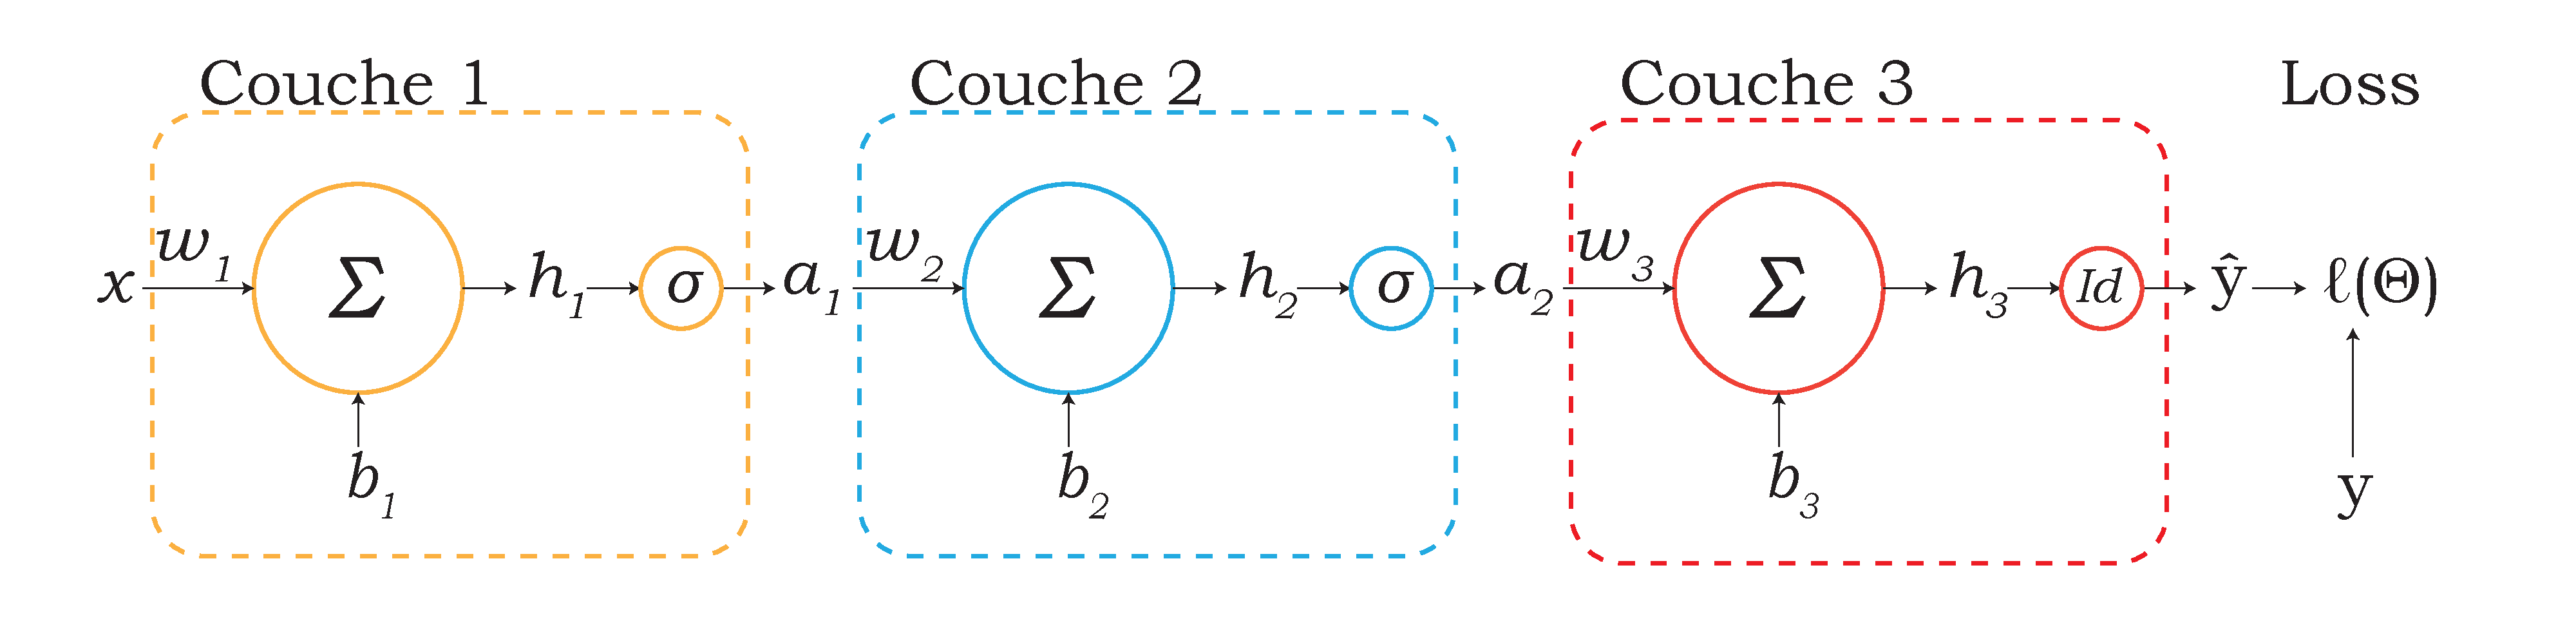
\includegraphics[width=\textwidth]{figures/3couches.pdf}
\end{figure}

\end{frame}

\begin{frame}{Exemple}{Backward pass}

    On commence par calculer la dérivée de la \textit{loss} par rapport à l'activité du dernier neurone du réseau $h_3$. La fonction d'activation est intégrée à ce calcul par simplicité.
    
    \begin{align*}
        \pdv{\ell}{h_3} &= \pdv{\ell}{\hat{y}} \cdot \odv{\hat{y}}{h_3} \\
                        &= \pdv{1/2(\hat{y} - y)^2}{\hat{y}} \cdot \odv{h_3}{h_3} \\
                        &= (\hat{y} - y) \cdot 1 \\
                        &= \varepsilon_3
    \end{align*}

    Ce terme, $\varepsilon_3$, représente l'erreur dans le contexte de la dernière couche, ici la couche 3.
    
\end{frame}

\begin{frame}{Exemple}{Backward pass -- couche 3}

On applique la règle de chaînage.
\vspace{1em}

    \begin{columns}
        \column{0.5\textwidth}
        Contribution de $w_3$ à l'erreur:

        \begin{align*}
            \pdv{\ell}{w_3} &= \underbrace{\pdv{\ell}{\hat{y}} \cdot \pdv{\hat{y}}{h_3}}_{\color{OliveGreen} \varepsilon_3} \cdot \pdv{h_3}{w_3} \\
            &= \varepsilon_3 \cdot \pdv{h_3}{w_3} = \varepsilon_3 \cdot \pdv{(w_3a_2 + b_3)}{w_3}\\
            &= \varepsilon_3 \cdot a_2
        \end{align*}

        \column{0.5\textwidth}
        Contribution de $b_3$ à l'erreur:

        \begin{align*}
            \pdv{\ell}{b_3} &= \underbrace{\pdv{\ell}{\hat{y}} \cdot \pdv{\hat{y}}{h_3}}_{\color{OliveGreen} \varepsilon_3} \cdot \pdv{h_3}{b_3} \\
            &= \varepsilon_3 \cdot \pdv{h_3}{b_3} = \varepsilon_3 \cdot \pdv{(w_3a_2 + b_3)}{b_3}\\
            &= \varepsilon_3 \cdot 1
        \end{align*}
        
    \end{columns}

\end{frame}


\begin{frame}{Exemple}{Backward pass -- couche 3 vers 2}

    On passe l'erreur dans la couche 3 pour la mettre à portée de la couche 2. On cherche donc à calculer la contribution des sorties de la couche 2 ($h_2$) à l'erreur actuelle ($\varepsilon_2$):
    \begin{align*}
        \pdv{\ell}{h_2} &= \pdv{\ell}{\hat{y}} \cdot \pdv{\hat{y}}{h_3} \cdot \pdv{h_3}{a_2} \cdot \pdv{a_2}{h_2} \\
            &= \varepsilon_3 \cdot \pdv{h_3}{a_2} \cdot \pdv{a_2}{h_2} = \varepsilon_3 \cdot \pdv{(w_3a_2 + b_3)}{a_2} \cdot \pdv{a_2}{h_2} \\
            &= \varepsilon_3 \cdot w_3 \cdot a_2(1-a_2) \\
            &= {\color{red} \varepsilon_2}
    \end{align*}

\end{frame}

\begin{frame}{Exemple}{Backward pass -- couche 2}

    \begin{columns}
        \column{0.5\textwidth}
        Contribution de $w_2$ à l'erreur:

        \begin{align*}
            \pdv{\ell}{w_2} &= \underbrace{\pdv{\ell}{\hat{y}} \cdot \pdv{\hat{y}}{h_3} \cdot \pdv{h_3}{a_2} \cdot \pdv{a_2}{h_2}}_{\color{red} \varepsilon_2} \cdot \pdv{h_2}{w_2} \\
            &= {\color{red} \varepsilon_2} \cdot \pdv{h_2}{w_2} \\
            &= {\color{red} \varepsilon_2} \cdot a_1
        \end{align*}

        \column{0.5\textwidth}
        Contribution de $b_2$ à l'erreur:

        \begin{align*}
            \pdv{\ell}{b_2} &= \underbrace{\pdv{\ell}{\hat{y}} \cdot \pdv{\hat{y}}{h_3} \cdot \pdv{h_3}{a_2} \cdot \pdv{a_2}{h_2}}_{\color{red} \varepsilon_2} \cdot \pdv{h_2}{b_2} \\
            &= {\color{red} \varepsilon_2} \cdot \pdv{h_2}{b_2} \\
            &= {\color{red} \varepsilon_2} \cdot 1
        \end{align*}
        
    \end{columns}

\end{frame}

\begin{frame}{Exemple}{Backward pass -- couche 2 vers 1}

    On passe l'erreur dans la couche 2 pour atteindre la couche 1 (contribution de $h_1$):

    \begin{align*}
        \pdv{\ell}{h_1} &= \underbrace{\pdv{\ell}{\hat{y}} \cdot \pdv{\hat{y}}{h_3} \cdot \pdv{h_3}{a_2} \cdot \pdv{a_2}{h_2}}_{\color{red} \varepsilon_2} \cdot \pdv{h_2}{a_1} \cdot \pdv{a_i}{h_1}\\
        &= {\color{red} \varepsilon_2} \cdot \pdv{h_2}{a_1} \cdot \pdv{a_i}{h_1} \\
        &= {\color{red} \varepsilon_2} \cdot w_1 \cdot a_1(1-a_1) \\
        &= {\color{blue} \varepsilon_1}
    \end{align*}

\end{frame}


\begin{frame}{Exemple}{Backward pass -- couche 1 et fin}

    Encore une (dernière) fois:

    \vspace{1em}

    \begin{columns}
        \column{0.5\textwidth}
        Contribution de $w_1$ à l'erreur:

        \begin{align*}
            \pdv{\ell}{w_1} &= {\color{blue} \varepsilon_1} \cdot \pdv{h_1}{w_1} \\
            &= {\color{blue} \varepsilon_1} \cdot x
        \end{align*}

        \column{0.5\textwidth}
        Contribution de $b_1$ à l'erreur:

        \begin{align*}
            \pdv{\ell}{b_1} &= {\color{blue} \varepsilon_1} \cdot \pdv{h_1}{b_1} \\
            &= {\color{blue} \varepsilon_1} \cdot 1
        \end{align*}
        
    \end{columns}
    
\end{frame}

\begin{frame}{\textit{Backward pass -- formule générique}}

La \textbf{backward pass} consiste donc premièrement à recalculer le $\varepsilon_l$ de la couche courante. Dans le cas où chaque couche possède $m_l$ neurones (donc $\w \in \mathbb{R}^{m_{l} \times m_{l+1}}$ et $\dim \mathbf{a}_l = \dim \mathbf{h}_l = m_{l}$):

\begin{align*}
    \underbrace{\nabla_{\mathbf{h}_l}\ell}_{\color{red}\text{gradient}} = \varepsilon_{l}^\intercal &= \mathbf{w}_{l+1} \cdot \varepsilon_{l+1} \odot \left(\odv{\mathbf{a}_{l}}{\mathbf{h}_{l}}\right)^\intercal
\end{align*}

On peut ensuite calculer la contribution des paramètres:

\begin{columns}
\column{0.5\textwidth}
    \begin{align*}
    \pdv{\ell}{\w_l} &= \varepsilon_l \cdot \mathbf{a}_l^\intercal = \nabla_{\mathbf{w}_l}\ell
\end{align*}
\column{0.5\textwidth}
\begin{align*}
    \pdv{\ell}{b_l} &= \varepsilon_l \cdot \mathbf{1} = \sum_i \varepsilon_{l,i}
\end{align*}
\end{columns}

\end{frame}

\begin{frame}{Descente de gradient}{Rappel}

Les gradients sont ensuite utilisés dans le cadre de l'algorithme de descente de gradient:

\begin{align*}
    \w_l &:= \w_l - \eta \nabla_{\w_l}\ell \\
    b_l &:= b_l - \eta \pdv{\ell}{b_l}
\end{align*}

avec $\eta$ un taux d'apprentissage fixé.

\textbf{Remarque}: il existe de nombreux autres algorithmes de descente de gradient, comme \textit{Adam} ou \textit{RMSProp}.

\end{frame}

\begin{frame}{Descente de gradient stochastique}{Definition}


\begin{columns}
    \column{0.5\textwidth}
\begin{block}{Boucle d'apprentissage (\textit{Training loop})}

Pour que l'algorithme de descente du gradient converge vers des valeurs $\Theta$ qui minimisent la \textit{loss}, on doit itérer \textit{forward} et \textit{backward pass} sur tout le jeu de données, plusieurs fois.

\vspace{1em}

On appelle une \textbf{\textit{epoch}} une itération complète du jeu de données.

\end{block}
    \column{0.5\textwidth}
    \begin{figure}
        \centering
        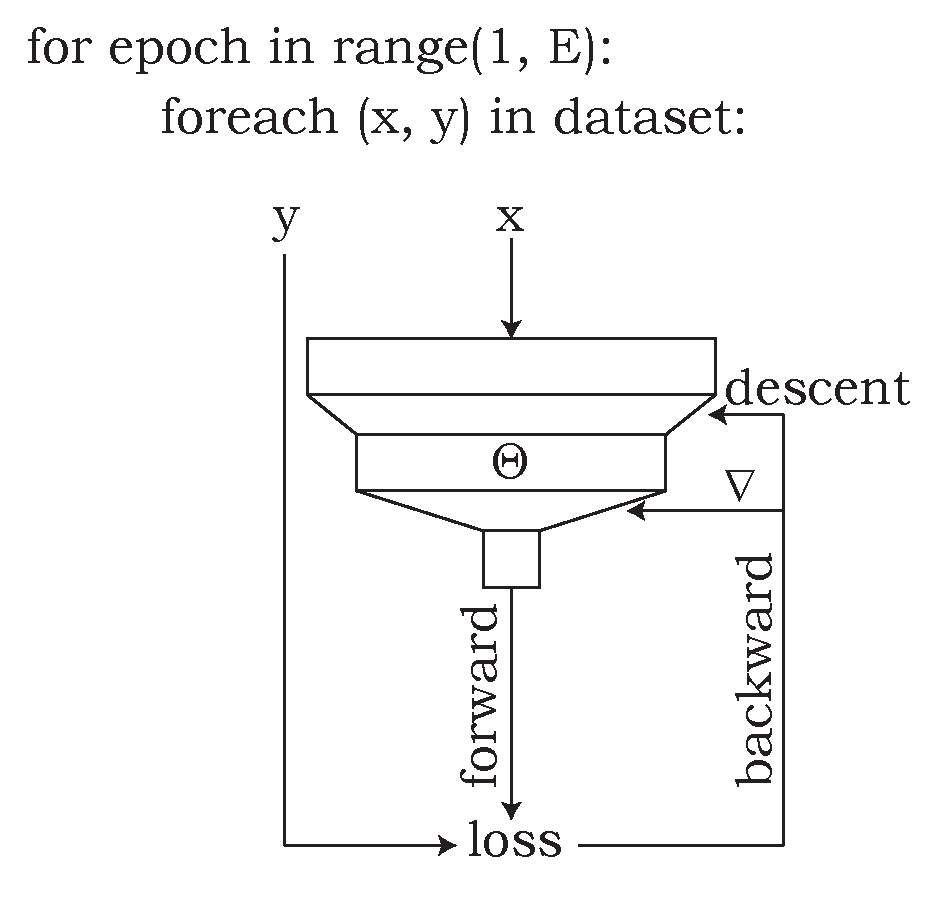
\includegraphics[width=0.7\textwidth]{figures/trainingloop.pdf}
    \end{figure}
\end{columns}

\end{frame}

\begin{frame}{Descente de gradient stochastique}{Définition}

\begin{columns}

\column{0.5\textwidth}
    On parle de descente de gradient stochastique lorsque, à chaque itération, le gradient est évalué sur une donnée $(\x_i, \y_i)$ tirée au hasard (sans replacement) dans le jeu de données.

\column{0.5\textwidth}

    \begin{figure}
        \centering
        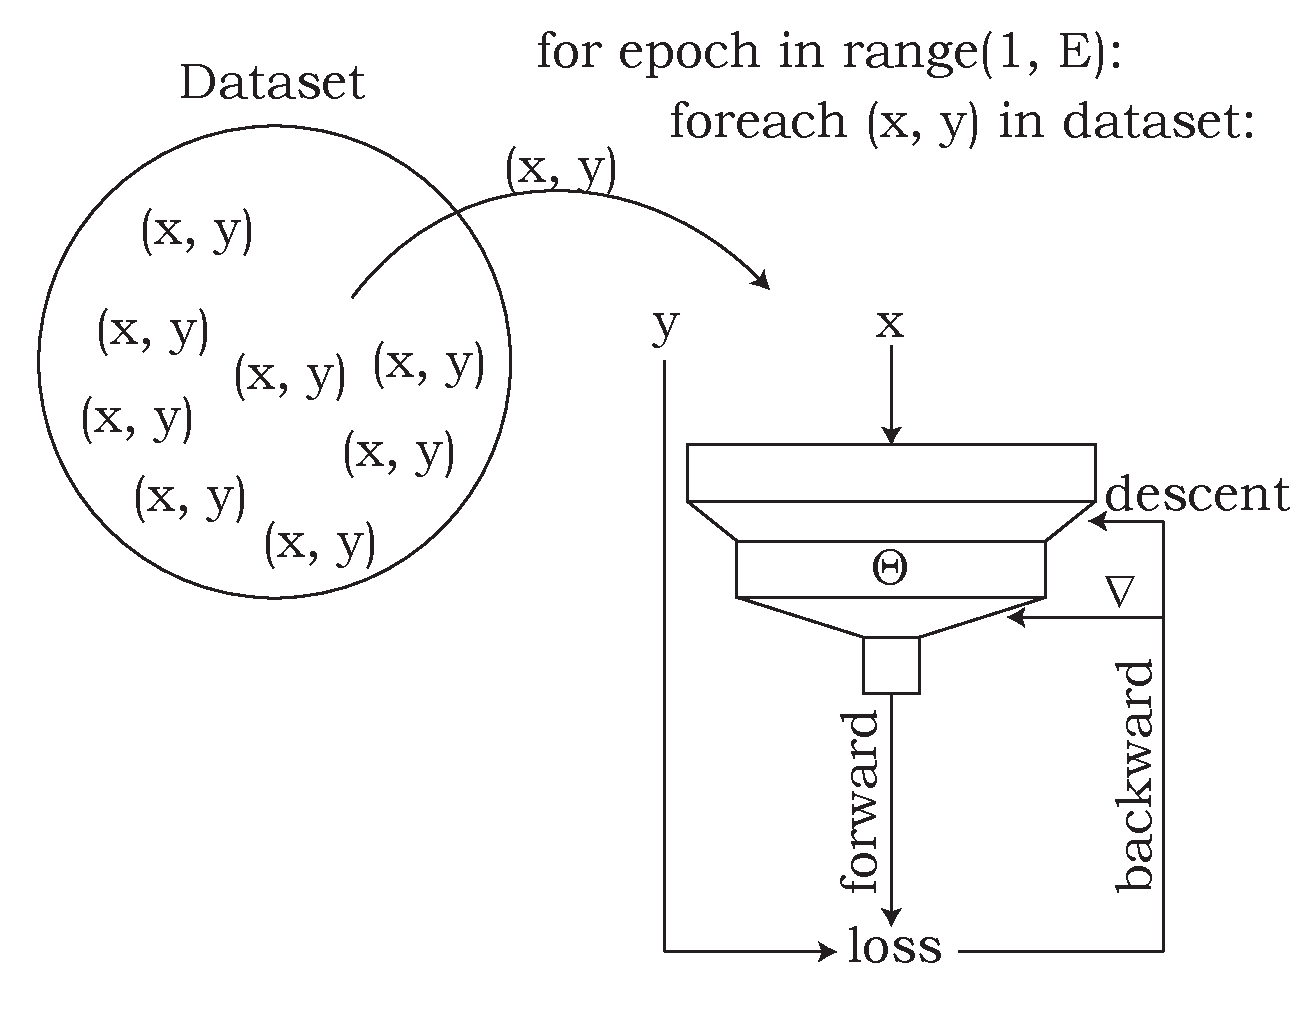
\includegraphics[width=\textwidth]{figures/sgd.pdf}
    \end{figure}

\end{columns}

    
\end{frame}

\begin{frame}{Descente de gradient stochastique}{Descente par \textit{batch}}

\begin{columns}

\column{0.4\textwidth}
    En pratique, pour accélerer les calculs et stabiliser l'apprentissage, on calcule la moyenne des gradients sur un \textbf{lot (\textit{batch})} aléatoire de points $(\x_i, \y_i)_{i=1\dots k}$, avec $k$ la taille d'un \textit{batch}.

\column{0.6\textwidth}

    \begin{figure}
        \centering
        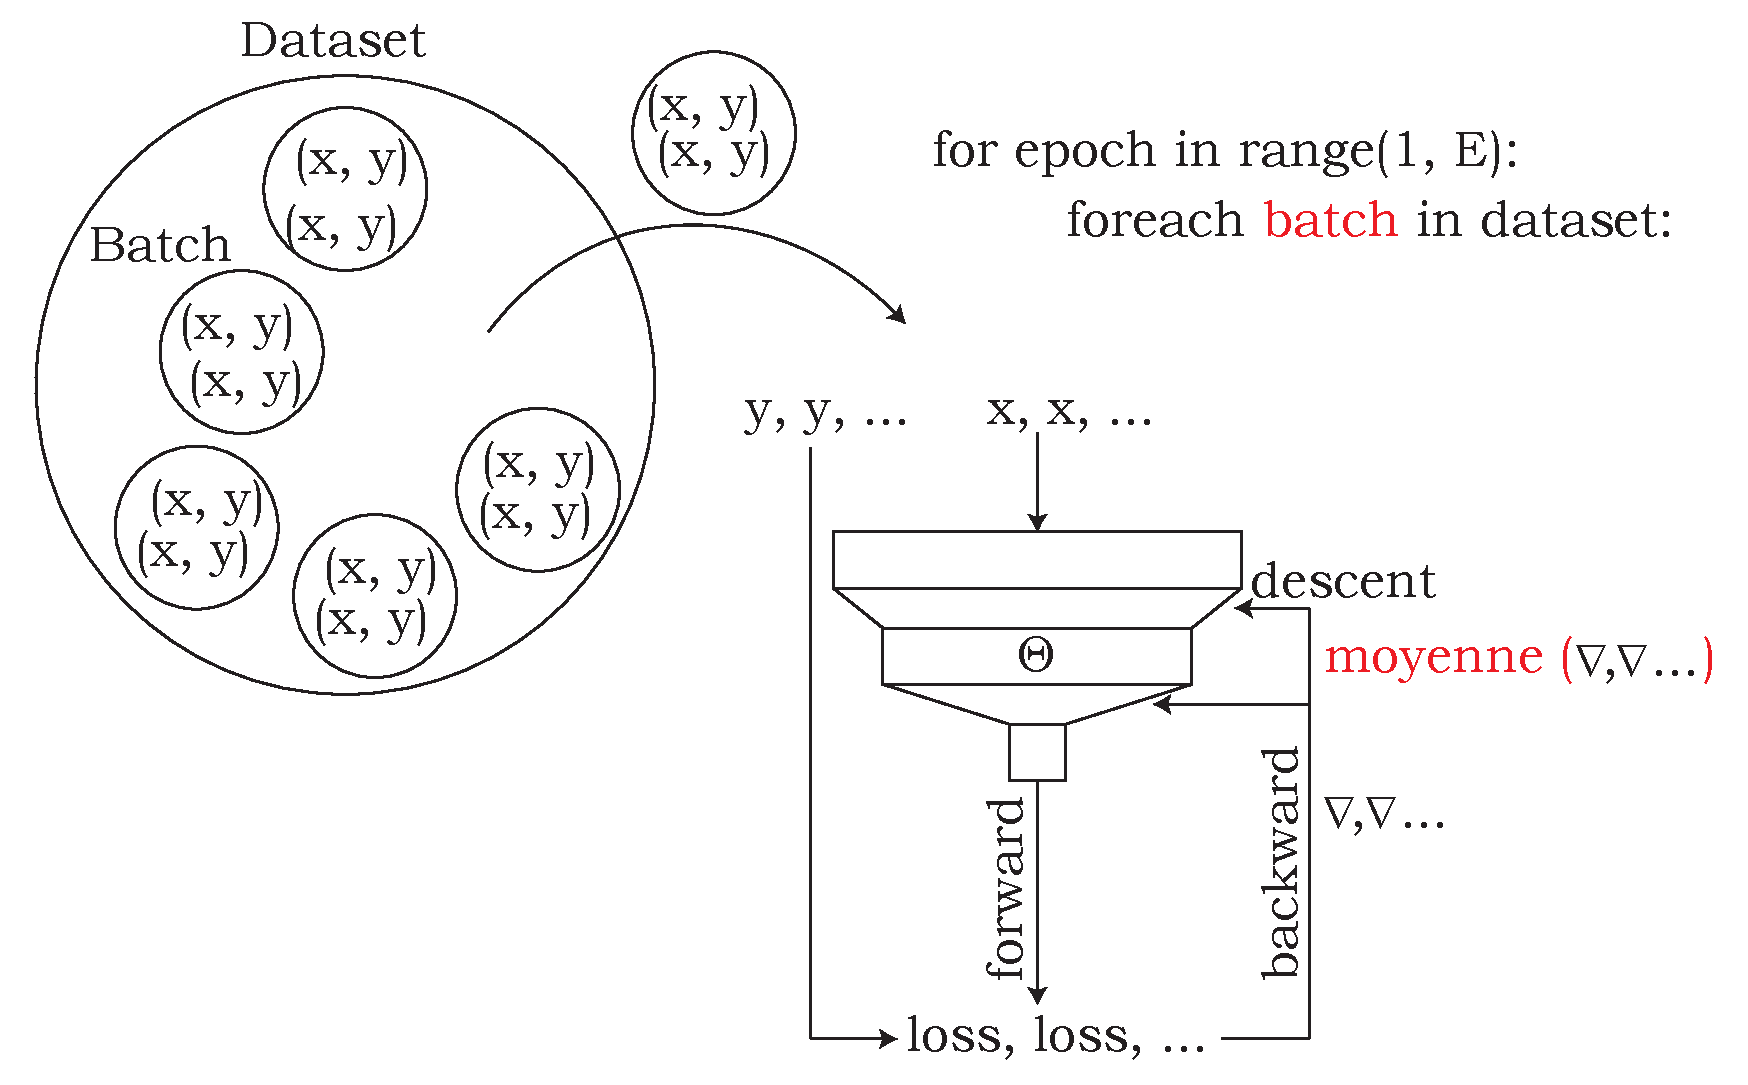
\includegraphics[width=\textwidth]{figures/sgd_batch.pdf}
    \end{figure}

\end{columns}
    
\end{frame}

\begin{frame}{Procédure d'entraînement}{Ne pas oublier ses bonnes manières}

Évidemment, ces techniques doivent être appliquées dans le cadre de travail du \textit{Machine Learning} étudié précédemment:

\begin{itemize}
    \item on définit des jeux de données de tests, de validation et d'entraînement pour mettre à jour le modèle et évaluer ses performances;
    \item les données sont formatées correctement (données numériques, \textit{one-hot encoding}...);
    \item plusieurs hypothèses (architectures de modèles) sont envisagées et comparées;
    \item \textit{etc}.
\end{itemize}
    
\end{frame}

\section{Implémentation et outils}

\begin{frame}{Graphes computationnels}

\begin{columns}

    \column{0.5\textwidth}

    Schéma du circuit d'un perceptron
    
    \begin{figure}
        \centering
        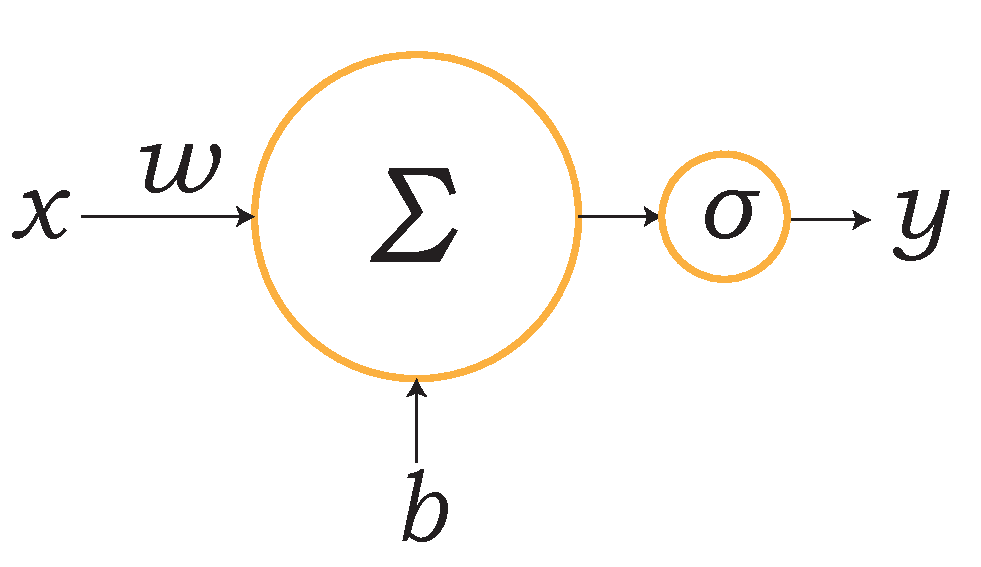
\includegraphics[width=\textwidth]{figures/nocompgraph.pdf}
    \end{figure}
        
    \column{0.5\textwidth}

    Graphe computationnel correspondant

    \begin{figure}
        \centering
        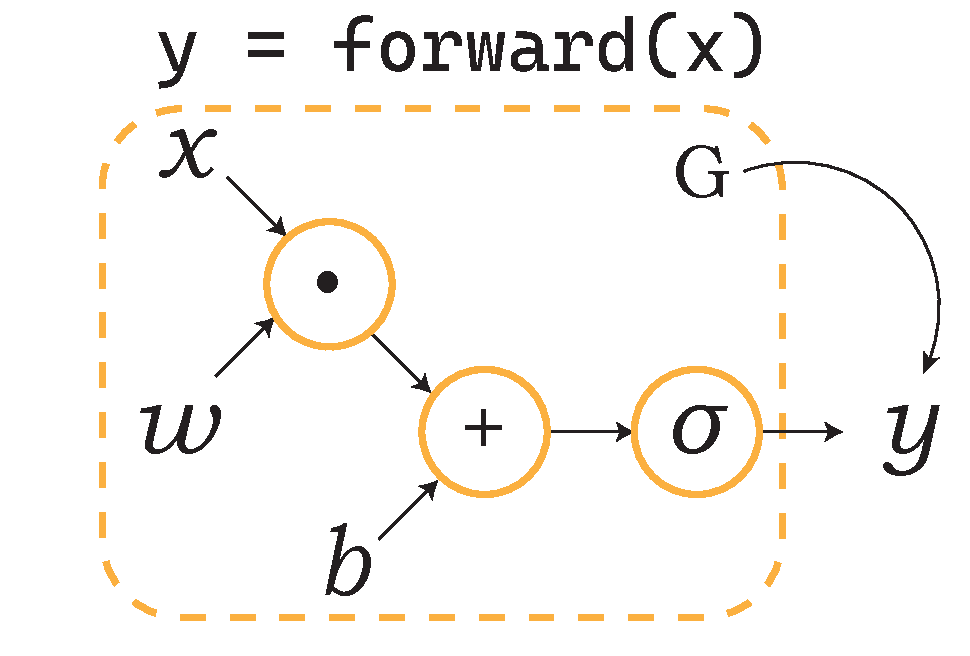
\includegraphics[width=\textwidth]{figures/compgraph.pdf}
    \end{figure}
    
\end{columns}

\end{frame}

\begin{frame}{Différentiation automatique (\textit{Autodiff})}


\begin{columns}

\column{0.5\textwidth}
    
\begin{figure}
    \centering
    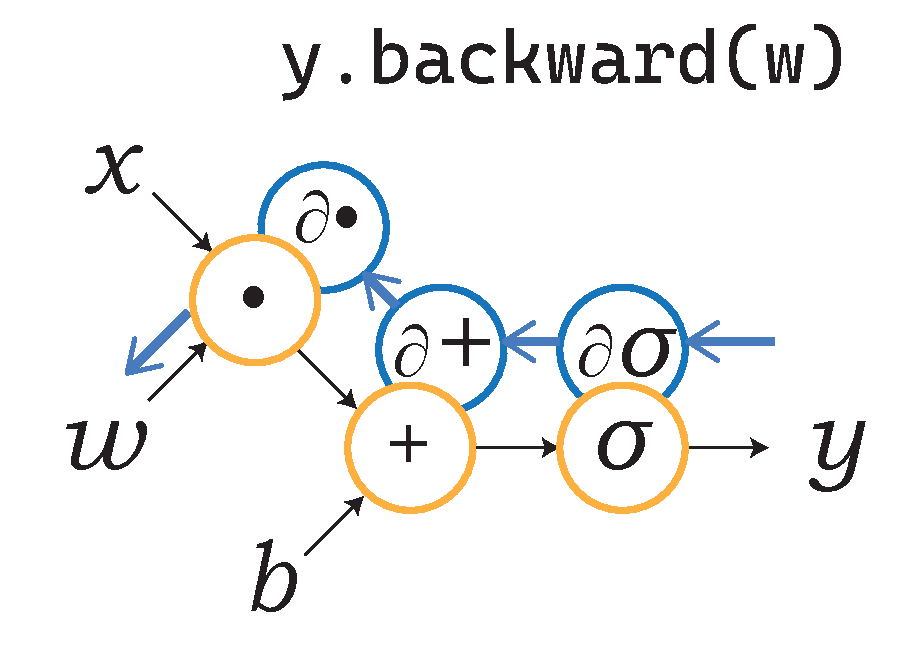
\includegraphics[width=\textwidth]{figures/autodiff.pdf}
\end{figure}

\column{0.5\textwidth}

Permet de propager le gradient grâce à la règle de chaînage \textbf{pour n'importe quelle opération} (opérateurs usuels, fonctions d'activation, et même du code Python grâce à certains outils).\par

A chaque opération est attachée une opération \textit{backward} qui calcule le gradient par chaînage.

\end{columns}

    
\end{frame}
    
\begin{frame}{Différentiation automatique (\textit{Autodiff})}{Implémentation (\textit{pytorch})}

\begin{figure}
    \centering
    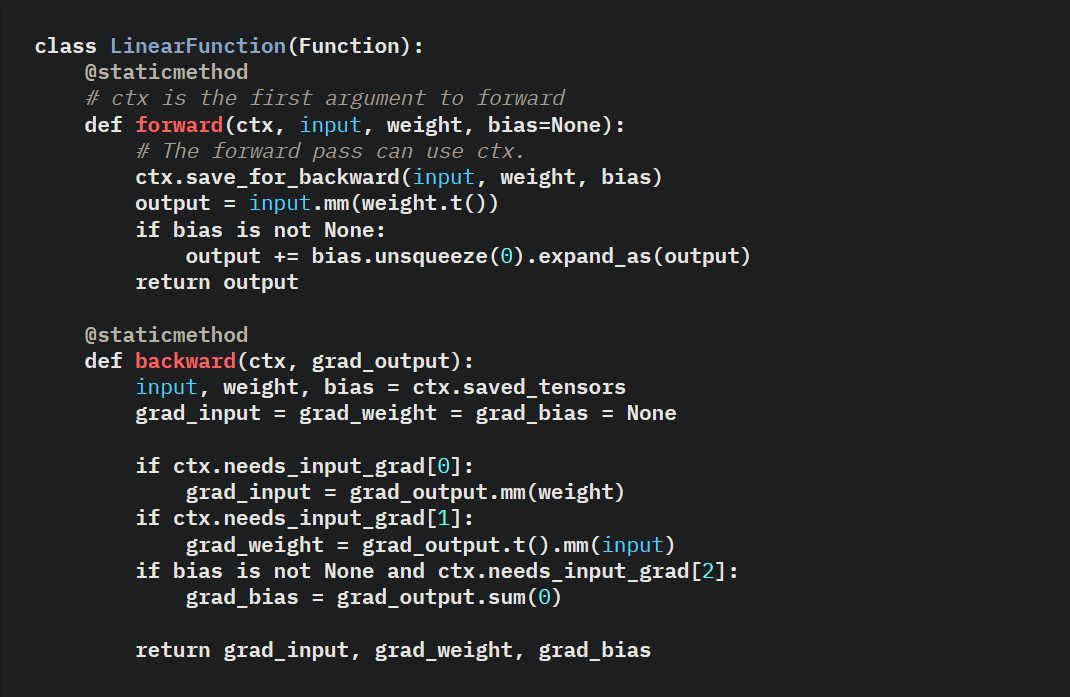
\includegraphics[width=0.6\textwidth]{figures/torchfunction.png}
\end{figure}
    
\end{frame}

\begin{frame}{Logiciels de \textit{deep learning}}{Une question de goût}

\begin{figure}
    \centering
    
\includegraphics[width=0.8\textwidth]{figures/frameworks.pdf}
\end{figure}
    
\end{frame}

\begin{frame}{Logiciels de \textit{deep learning}}{Celui qui ne nous laissera jamais tomber}

\begin{figure}
    \centering
    
\includegraphics[width=0.5\textwidth]{figures/sklearnlogo.png}
\end{figure}

\end{frame}

\begin{frame}{(Petite démonstration ?)}
    
\end{frame}

\begin{frame}{Au prochain épisode}

    \begin{itemize}
        \item TD6 -- Entraînement de réseaux de neurones \textit{from scratch}
    \end{itemize}

    \begin{block}{Lectures complémentaires}

    \begin{itemize}
        \item Minsky, M. (1961). Steps Toward Artificial Intelligence.  \textit{Proc. IRE}
        \item Rumelhart, D., Hinton, G. & Williams, R. (1986). Learning representations by back-propagating errors. \textit{Nature}
        \item Goodfellow, I., Bengio, Y., & Courville, A. (2016). Deep learning. \textit{MIT press.} (https://www.deeplearningbook.org/)
        \item Bishop, C. (2006). Pattern recognition and machine learning. \textit{Springer} (online)
        \item Olah, C., colah's blog, https://colah.github.io/
    \end{itemize}


        
    \end{block}

\end{frame}

\end{document}
